% ICSE 2027 NIER submission -- 4 pages main text + 1 page references.
% The CfP mandates exactly \documentclass[10pt,conference]{IEEEtran};
% the unofficial "anonymous" option was removed (IEEEtran ignores it).
\documentclass[10pt,conference]{IEEEtran}
\IEEEoverridecommandlockouts

% --- Symbols & Custom Marks ---
\usepackage{pifont}
\newcommand{\cmark}{\ding{51}}
\newcommand{\xmark}{\ding{55}}
\newcommand{\pmark}{\ding{109}} % partial coverage

% --- Core Packages ---
\usepackage{cite}
\usepackage{amsmath,amssymb,amsthm,amsfonts}
\usepackage[expansion=false]{microtype}
\usepackage{booktabs, multirow}
\usepackage{xcolor}
\usepackage{graphicx}
\usepackage{textcomp}

% --- Visualization & Plots ---
\usepackage{tikz}
\usepackage{pgfplots}
\pgfplotsset{compat=1.18}
\usepgfplotslibrary{statistics,groupplots}
\usetikzlibrary{arrows.meta,positioning,shapes.geometric,automata,fit,backgrounds,calc}

% --- Algorithms & Code ---
\usepackage{algorithm}
\usepackage{algpseudocode}
\usepackage{listings}

% --- Layout & Utility ---
\usepackage{mdframed}
\usepackage{enumitem}
\usepackage{hyperref}
\usepackage{cleveref}
\hypersetup{hidelinks}

% --- Theorem environments ---
\theoremstyle{definition}
\newtheorem{definition}{Definition}
\newtheorem{example}{Example}[section]
\newtheorem{problem}{Problem Statement}[section]
\newtheorem{assumption}{Assumption}
\renewcommand{\theassumption}{A\arabic{assumption}}
\theoremstyle{plain}
\newtheorem{theorem}{Theorem}[section]
\newtheorem{proposition}{Proposition}
\newtheorem{lemma}{Lemma}[section]
\newtheorem{corollary}{Corollary}[section]
\theoremstyle{remark}
\newtheorem{remark}{Remark}[section]

% --- Running-example box ---
\newmdenv[
  backgroundcolor=gray!7,
  linecolor=black!25, linewidth=0.5pt,
  topline=true, bottomline=true, leftline=true, rightline=true,
  innertopmargin=4pt, innerbottommargin=4pt,
  innerleftmargin=6pt, innerrightmargin=6pt,
  skipabove=6pt, skipbelow=6pt
]{runbox}

% --- Listing style (view-metamodel / rule snippets) ---
\lstdefinelanguage{ATL}{
  morekeywords={module,create,from,rule,to,lazy,unique,helper,def,
                context,uses,thisModule,and,or,not,in},
  morekeywords=[2]{@llm,@check},
  sensitive=true, morecomment=[l]{--}, morestring=[b]'}
\lstset{frame=single, backgroundcolor=\color{gray!5},
        basicstyle=\ttfamily\scriptsize, breaklines=true,
        showstringspaces=false, numbers=none, upquote=true,
        keywordstyle=\bfseries, keywordstyle={[2]\bfseries\color{purple}},
        commentstyle=\itshape\color{black!60},
        aboveskip=4pt, belowskip=2pt, xleftmargin=2pt, xrightmargin=2pt}

% --- Custom Commands ---
\newcommand{\finding}[1]{\smallskip\noindent\textbf{Finding:} \textit{#1}\smallskip}
\algnewcommand{\LineComment}[1]{\State \(\triangleright\) \textit{#1}}
\algnewcommand\algorithmicinput{\textbf{Input:}}
\algnewcommand\algorithmicoutput{\textbf{Output:}}
\algnewcommand\Input{\item[\algorithmicinput]}
\algnewcommand\Output{\item[\algorithmicoutput]}

% --- Math shorthands (AgentM2M) ---
\newcommand{\tool}{\textsc{AgentM2M}}
\newcommand{\devteam}{\textsc{DevTeam}}
\newcommand{\MM}{\mathit{MM}}
\newcommand{\Mods}[1]{\mathcal{M}(#1)}
\newcommand{\AllMods}[1]{\mathcal{M}^{\ast}(#1)}
\newcommand{\TL}{\mathit{TL}}
\newcommand{\Team}{\mathit{Team}}
\newcommand{\team}{\mathcal{T}}
\newcommand{\fwd}[1]{\overrightarrow{#1}}
\newcommand{\bwd}[1]{\overleftarrow{#1}}
\newcommand{\str}{\mathrm{str}}
\newcommand{\sem}{\mathrm{sem}}
\newcommand{\NL}{\mathsf{NL}}
\newcommand{\Dist}[1]{\mathcal{D}(#1)}
\newcommand{\den}[1]{[\![#1]\!]}
\newcommand{\cls}[1]{\textsf{#1}}
\newcommand{\RC}[1]{\textbf{RC#1}}
\newcommand{\code}[1]{\texttt{#1}}
\newcommand{\step}[1]{\textcircled{\scriptsize #1}}
\newcommand{\fp}{\mathit{fp}}
\newcommand{\Obl}{\mathit{Obl}}
\DeclareRobustCommand{\tracemark}{\tikz[baseline=-0.6ex]\node[draw,diamond,fill=black!70,inner sep=1.1pt]{};}

\newcommand{\ahsays}[1]{{\color{purple}{\bf AH:} #1}}
\newcommand{\fixme}[1]{{\color{red}[#1]}}
\definecolor{fixedgreen}{RGB}{0,128,0}
\newcommand{\fixed}[1]{{\color{fixedgreen}#1}}
% --- drafting aids for unmeasured results (remove before submission) ---
\newcommand{\ph}{{\color{red}\textbf{--.-}}}     % unmeasured number
\newcommand{\hyp}[1]{{\color{blue}#1}}           % result-dependent sentence
\newif\ifplaceholderdata \placeholderdatatrue     % set false once plots hold data
\newcommand{\phwatermark}{\ifplaceholderdata
  \node[red, opacity=0.55, font=\bfseries\scriptsize, rotate=12]
  at (rel axis cs:0.5,0.55) {PLACEHOLDER DATA};\fi}

\begin{document}

\title{Towards Deterministic Structure for Stochastic Agents: M2M Transformations for Agentic Collaborations}

% --- Double-anonymous review: keep the author block commented out. ---
% \author{\IEEEauthorblockN{Majid Babaei}
% \IEEEauthorblockA{\textit{School of Computing} \\
% \textit{University of the Fraser Valley}\\
% BC, Canada \\
% majid.babaei@ufv.ca}
% }

\maketitle

\begin{abstract}
Teams of LLM agents fail less because individual agents are weak than
because the \emph{glue} between them is weak: hand-offs are free text,
nothing records which artifacts correspond, and team structure is frozen at
design time. We argue that this glue is a problem model-driven engineering
has already solved for deterministic tools, and we propose \tool{}, which
treats every hand-off between agents as a model-to-model (M2M) transformation
in the style of ATL. Each agent owns a view model conforming to its own
metamodel; a hand-off is a set of declarative matched rules whose
\emph{structure}---matching, element creation, reference resolution and trace
links---is executed by a deterministic engine, while the LLM is confined to
\emph{stochastic bindings} that fill attribute values from a bounded source
footprint and are accepted only after validation. The team becomes a network
of transformations whose generated trace models drive consistency
restoration, and whose runtime evolution is itself a higher-order
transformation. We show that this separation yields three properties that
free-text teams lack---structural independence from LLM sampling, sound change
impact, and a bounded residual error per binding---relate them to 11 of the
14 MAST failure modes (5 fully, 6 partially), and outline the evaluation that
will test them.
\end{abstract}

\begin{IEEEkeywords}
LLM-based multi-agent systems, model-to-model transformation, ATL,
traceability, bidirectional transformations, higher-order transformations
\end{IEEEkeywords}

\section{Introduction}\label{sec:introduction}

LLM-based agents are moving from single assistants to \emph{teams} of
specialized agents that jointly analyze, design, implement, and test
software~\cite{he2025lma}. Role-based frameworks assign agents the roles of a
software organization~\cite{hong2024metagpt,qian2024chatdev,tao2024magis},
while conversation- and graph-centric frameworks let developers wire arbitrary
topologies~\cite{wu2024autogen,li2023camel,chen2024agentverse}. The promise is
that specialization, context isolation, and cross-examination make a team more
reliable than a single agent.

The empirical record is sobering. Cemri et al.\ analyzed more than 1{,}600
annotated traces of seven multi-agent frameworks and derived the MAST taxonomy
of 14 failure modes~\cite{cemri2025mast}. Gains over single-agent baselines
are often minimal, and 44.2\% of the failure-mode occurrences they report fall
into \emph{system design issues}, 32.3\% into \emph{inter-agent misalignment},
and 23.5\% into \emph{task verification}. Their case studies also show that
changing the \emph{structure} of a team---e.g., letting ChatDev's CEO agent
have the final say---can raise task success substantially without changing the
model~\cite{cemri2025mast}.

\smallskip\noindent\textbf{Problem analysis.} To identify what a
coordination layer could fix, we mapped each MAST failure mode to the
coordination deficit it manifests (Table~\ref{tab:mast}). This is an
analytical mapping based on the published mode definitions, not a systematic
literature review; the mapping and its rationale are part of our
artifact (Section~\ref{sec:data}). Three deficits emerge:

\noindent\textbf{P1: Lossy hand-offs between heterogeneous views.} Each agent
reasons over its own representation---user stories, components, code edits,
test verdicts---but hand-offs are free text re-interpreted by an LLM at every
step. Information is dropped or hallucinated silently (FM-1.4, 2.1, 2.4, 2.5).

\noindent\textbf{P2: No consistency maintenance or traceability under
change.} Collaboration is iterative, yet nothing records which artifacts
\emph{correspond}; agents act on stale artifacts and repeat work, and
verification is detached from what it should verify (FM-1.3, 3.2, 3.3).

\noindent\textbf{P3: Rigid collaboration structures.} Roles, topology, and
hand-off protocols are fixed at design time; adapting a team at runtime
requires re-engineering the glue between agents by hand (FM-1.2, 1.5, and the
structural interventions of~\cite{cemri2025mast}).

Table~\ref{tab:mast} also makes explicit which modes a coordination layer
\emph{cannot} address, such as disobeying the task specification (FM-1.1) or
failing to ask for clarification (FM-2.2); we return to them in
Section~\ref{subsec:discussion}.

\begin{table}[t]
\centering
\caption{Analytical mapping of MAST failure modes~\cite{cemri2025mast} to
coordination deficits and the \tool{} mechanism targeting them
(\cmark\ targeted, \pmark\ partially, \xmark\ not targeted).}
\label{tab:mast}
\footnotesize
\setlength{\tabcolsep}{3pt}
\begin{tabular}{@{}l l l c@{}}
\toprule
MAST mode & Deficit & \tool{} mechanism & Cov. \\
\midrule
1.1 Disobey task spec.        & --  & -- & \xmark \\
1.2 Disobey role spec.        & P3  & write rights $\omega$ & \pmark \\
1.3 Step repetition           & P2  & obligations, version stamps & \pmark \\
1.4 Loss of conv.\ history    & P1  & persistent view models & \cmark \\
1.5 Unaware of termination    & P3  & acceptance predicate $\varphi$ & \pmark \\
2.1 Conversation reset        & P1  & persistent view models & \cmark \\
2.2 Fail to ask clarification & --  & -- & \xmark \\
2.3 Task derailment           & P2  & rule guards, footprints & \pmark \\
2.4 Information withholding   & P1  & matched rules, coverage & \cmark \\
2.5 Ignored other's input     & P1  & obligations from traces & \cmark \\
2.6 Reasoning-action mismatch & --  & -- & \xmark \\
3.1 Premature termination     & P2  & acceptance predicate $\varphi$ & \pmark \\
3.2 No/incompl.\ verification & P2 & trace links to tests & \cmark \\
3.3 Incorrect verification    & P2  & executable validators & \pmark \\
\bottomrule
\end{tabular}
\end{table}

\smallskip\noindent\textbf{Existing remedies.} Interoperability protocols such
as MCP and A2A~\cite{mcp2024,a2a2025} standardize \emph{how} messages are
transported, not \emph{what} they mean or how artifacts relate. Structured
documents~\cite{hong2024metagpt} and schema-validated shared
state~\cite{zhang2026patchboard} make outputs well-formed, but a single
shared schema removes heterogeneity by fiat and leaves relations
\emph{between} perspectives implicit. Automated agent-system
design~\cite{zhuge2024gptswarm,hu2025adas,zhang2025aflow} searches topologies
offline, without guarantees about what flows along the edges.

\smallskip\noindent\textbf{Key insight.} Managing heterogeneous views,
relating them explicitly, keeping them consistent under change, and evolving
them at runtime are core concerns of model-driven engineering (MDE): view-based
development~\cite{klare2021vitruvius,bruneliere2019views},
bidirectional transformations (bx)~\cite{czarnecki2009bx,stevens2010qvt}
and their networks~\cite{stevens2020networks,klare2023termination},
models@run.time~\cite{blair2009runtime}, and higher-order transformations
(HOTs)~\cite{tisi2009hot}. What these theories do \emph{not} cover is the
defining property of agent teams: the transformations between views are
performed by stochastic LLMs, and the team itself changes while it
runs.

\smallskip\noindent\textbf{Our approach.} \tool{} treats every hand-off as an
M2M transformation in the sense of ATL~\cite{jouault2008atl}, and splits each
transformation rule along a line that ATL's execution model already draws.
Everything ATL guarantees deterministically such as matching source patterns,
creating target elements, resolving references through traceability, stays
with a deterministic engine. Only what genuinely needs an LLM, like the
\emph{value} of a natural-language or code attribute, is delegated, as a
\emph{stochastic binding} evaluated over a declared source footprint and
accepted only after validation. Trace links, which ATL keeps
transiently~\cite{jouault2005traceability}, are persisted as trace
models~\cite{vara2014metagem} and become the correspondences of a bx network;
changing the team is a HOT over a team model kept at runtime. 

\noindent\textbf{Our
contributions.} \textbf{(C1)} the formulation of agent teams as networks of
hybrid deterministic/stochastic M2M transformations (Section~\ref{sec:approach});
\textbf{(C2)} three properties with proof sketches that follow from ATL's
semantics (Section~\ref{sec:properties}); and \textbf{(C3)} an evaluation
protocol with falsifiable predictions, grounded in MAST
(Section~\ref{sec:eval}).

\section{AgentM2M}\label{sec:approach}

\begin{figure}[t]
\centering
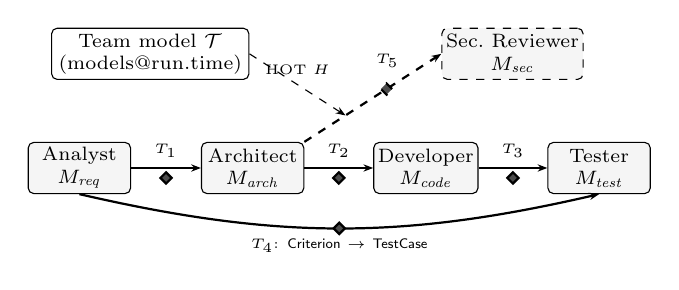
\begin{tikzpicture}[
  font=\scriptsize, >={Stealth[length=3.5pt]},
  view/.style={draw, rounded corners=2pt, fill=gray!8, minimum width=13mm,
               minimum height=6.5mm, align=center, inner sep=1.5pt},
  tr/.style={->, thick},
  trace/.style={draw, diamond, fill=black!70, inner sep=1.1pt},
  lbl/.style={font=\tiny, align=center}]
  \node[view] (req)  at (0,0)    {Analyst\\$M_{\mathit{req}}$};
  \node[view] (arch) at (2.2,0)  {Architect\\$M_{\mathit{arch}}$};
  \node[view] (code) at (4.4,0)  {Developer\\$M_{\mathit{code}}$};
  \node[view] (test) at (6.6,0)  {Tester\\$M_{\mathit{test}}$};
  \foreach \a/\b/\n in {req/arch/1, arch/code/2, code/test/3}{
    \draw[tr] (\a) -- node[above, lbl] {$T_{\n}$}
                      node[below=1pt, trace] {} (\b);}
  \draw[tr] (req.south) to[bend right=13]
     node[below, lbl] {$T_4$: \cls{Criterion} $\to$ \cls{TestCase}}
     node[pos=0.5, trace] {} (test.south);
  \node[view, fill=white, text width=24mm] (team) at (0.9,1.45)
     {Team model $\team$\\(models@run.time)};
  \node[view, dashed] (sec) at (5.5,1.45) {Sec.\ Reviewer\\$M_{\mathit{sec}}$};
  \draw[tr, dashed] (arch.north east) -- node[pos=0.6, trace] {}
     node[pos=0.75, above left=-1pt, lbl] {$T_5$} (sec.west);
  \draw[->, dashed] (team.east) -- node[above, lbl] {HOT $H$}
     ($(arch.north east)!0.3!(sec.west)$);
\end{tikzpicture}
\caption{\devteam{} as a megamodel. Agents own view models; hand-offs
$T_i$ are hybrid M2M transformations whose trace models
(\tracemark) persist. At
runtime, a HOT over the team model adds a reviewer and its hand-off $T_5$
(dashed).}
\label{fig:overview}
\end{figure}

\subsection{Views, hand-offs, and the team megamodel}

Following ATL's
architecture~\cite{jouault2008atl}, every artifact exchanged in a team is a
model $M_i \in \Mods{\MM_i}$ conforming to a view metamodel $\MM_i$ owned by
agent $a_i$. A \emph{team} is a megamodel
$\team = (A, V, \mathbf{T}, \omega, \varphi)$: agents $A$, views
$V=\{\MM_i\}$, hand-off transformations $\mathbf{T}$, write rights
$\omega : A \to 2^{V}$, and an acceptance predicate $\varphi$
(Fig.~\ref{fig:overview}). A hand-off $T_{ij} : \Mods{\MM_i} \to
\Mods{\MM_j}$ is a set of ATL-style rules $r=(p_r, g_r, t_r, B_r)$: a source
pattern $p_r$ with OCL guard $g_r$, a target pattern $t_r$, and bindings
$B_r$. $\omega$ transfers ATL's execution discipline to agents:
an agent reads upstream views (sources are read-only) and writes only its own
(targets are write-only), which is what makes matching stable and the result
independent of rule scheduling in ATL.
Multi-source hand-offs ($n{:}m$, e.g., the Developer reads both
$M_{\mathit{req}}$ and $M_{\mathit{arch}}$) are declared as in
ATL, with several \code{from} models.

\subsection{Hybrid rules: structural vs.\ stochastic bindings}

\begin{definition}[Hybrid hand-off]\label{def:hybrid}
A hand-off $T=(R^{\str},B^{\sem},\mathcal{L},\mathit{chk})$ consists of the
structural part $R^{\str}$ (patterns, guards, target patterns, and OCL
bindings of all rules), stochastic bindings $B^{\sem}$, an LLM $\mathcal{L}$
inducing a distribution $\Dist{\pi}$ over values for each prompt $\pi$, and a
validator $\mathit{chk}_b$ per $b\in B^{\sem}$.
\end{definition}

\noindent Accordingly, each rule's bindings are partitioned into
$B_r = B_r^{\str} \uplus B_r^{\sem}$. Structural bindings are ordinary OCL expressions, including
references that ATL resolves through its trace (e.g., \code{component <-
s.epic} yields the component \emph{generated from} \code{s.epic}). A stochastic
binding $b \in B_r^{\sem}$ has the form \code{f <- @llm(prompt, e)}, where
the OCL expression $e$ defines the \emph{footprint} $\fp_b(m)$ of match $m$.
Its value is sampled as $v \sim \Dist{\mathit{prompt} \oplus
\den{e}_m}$---the prompt is built \emph{only} from the footprint---and a
validator \code{@check} (a type/OCL constraint, a parser, or an executable
oracle) decides acceptance; on rejection the engine resamples up to $k$
times, then raises an escalation. Free-text output that must become model
elements goes through \textsc{Lift}, a text-to-model step that is rejected
unless the result conforms to $\MM_j$. Stochastic bindings are restricted to
primitive-typed attributes (strings, code bodies), never references.

\begin{runbox}
\noindent\textbf{Running example (\devteam).}
The Analyst's user stories become the Architect's operations:
\begin{lstlisting}[language=ATL, caption={The \tool{} rule dialect used throughout this evaluation.}, label={lst:rules}]
module Req2Arch;
create OUT : Arch from IN : Req;
rule Story2Operation {
 from s : Req!UserStory
          (s.status = #accepted)  -- guard
 to  op : Arch!Operation (
   name      <- s.id.toOpName(),  -- structural
   component <- s.epic,     -- resolved via trace
   signature <- @llm('Derive an API signature',
                     s.criteria),  -- footprint
   @check signature.parses()
          and signature.params->notEmpty() ) }
\end{lstlisting}
\noindent A second hand-off $T_4$ (\code{Criterion2TestCase}) maps each
acceptance criterion to a test case whose oracle body is a stochastic
binding with footprint \code{c.text}; its validator requires that the oracle
compiles and fails on a stub. Every accepted story thus has an operation and
every criterion a test (FM-2.4, 3.2), and both are linked by trace.
\end{runbox}

\subsection{Trace models, change, and obligations}

ATL records, for each rule application, which target elements were produced
from which match~\cite{jouault2005traceability}; MeTAGeM-Trace makes these
links a first-class, persistent trace model~\cite{vara2014metagem}. \tool{}
persists $\TL_{ij} \subseteq \mathit{Match}(M_i) \times M_j \times R$,
annotated, for every accepted stochastic binding, with its footprint and a
version stamp: a digest of $\den{e}_m$ at acceptance time.
Algorithm~\ref{alg:handoff} extends ATL's standard execution
scheme accordingly.

\begin{algorithm}[t]
\caption{Executing a hybrid hand-off $T_{ij}$}\label{alg:handoff}
\footnotesize
\begin{algorithmic}[1]
\Input source $M_i$ (read-only), trace $\TL_{ij}$, budget $k$
\Output target $M_j$, updated $\TL_{ij}$, escalations $E$
\State $\mathit{Mt}\gets\{(r,m)\mid m\models p_r\wedge g_r(m)\}$
  \Comment{fixed: $M_i$ is read-only}
\ForAll{$(r,m)\in\mathit{Mt}$ without a link in $\TL_{ij}$}
  \State create the elements $t$ of $t_r$; $\TL_{ij}\gets\TL_{ij}\cup\{(m,t,r)\}$
\EndFor
\State delete links $(m,t,r)$ with $(r,m)\notin\mathit{Mt}$, and their $t$
\State evaluate all $B^{\str}$; resolve source references via $\TL_{ij}$
\ForAll{$(m,t,r)\in\TL_{ij}$, $b\in B_r^{\sem}$ with
  $\mathit{stamp}(t,b)\neq\#\den{e_b}_m$}
  \State $\pi\gets\mathit{prompt}_b\oplus\den{e_b}_m$
    \Comment{footprint only}
  \State sample $v\sim\Dist{\pi}$ until $\mathit{chk}_b(v)$, at most $k$ times
  \If{accepted} $t.f_b\gets v$; $\mathit{stamp}(t,b)\gets\#\den{e_b}_m$
  \Else\ $E\gets E\cup\{(t,b)\}$ \Comment{escalate, never loop}
  \EndIf
\EndFor
\end{algorithmic}
\end{algorithm}
 When an agent edits its view (change $\Delta$ on $M_i$),
the engine (i)~re-runs $R^{\str}$ incrementally, which is cheap and
deterministic, and (ii)~emits \emph{obligations}
\begin{align*}
\Obl(\Delta)=\{(t,b)\mid{}&(m,t,r)\in \TL_{ij},\ b\in B_r^{\sem},\\
  &\fp_b(m)\cap \mathit{foot}(\Delta)\neq\emptyset\},
\end{align*}
each addressed to the agent $a$ with $\MM_j \in \omega(a)$; in
Algorithm~\ref{alg:handoff} these are exactly the stamp mismatches. Obligations
propagate along the network like consistency restoration in bx
networks~\cite{stevens2020networks}; we schedule them with the conservative
strategy of Klare and Gleitze, which is proven to terminate at the price of
occasionally failing~\cite{klare2023termination}, and escalate failures
rather than looping (FM-1.3). The team is done when $\varphi$ holds: every
match is covered by a trace link, no obligation is open, all version stamps
are fresh, and all validators pass (FM-1.5, 3.1).

\begin{runbox}
\noindent\textbf{Change scenario.} The Analyst tightens a criterion of story
\code{S2}. The trace model yields exactly
$\Obl=\{(\mathit{op}_{S2},\code{signature}),(\mathit{tc}_{S2.1},\code{oracle})\}$;
the Architect and Tester receive them. Once the Architect re-samples the
signature, $T_2$'s stamp check turns the dependent code edit into an
obligation for the Developer; no unrelated artifact is regenerated.
\end{runbox}

\subsection{Evolving the team with higher-order transformations}

MeTAGeM-Trace develops transformations model-driven: a high-level relation
model between metamodels is refined by HOTs into executable ATL that also
generates traces~\cite{vara2014metagem}. \tool{} applies the same chain at
runtime. The team model $\team$ is kept causally connected to the running
team (models@run.time~\cite{blair2009runtime}); a team change, e.g.,
\emph{add a Security Reviewer with view $\MM_{\mathit{sec}}$ related to
\cls{Operation}}, is a relation model that a HOT~\cite{tisi2009hot} turns into
a trace-generating hand-off $T_{\mathit{arch},\mathit{sec}}$, a new entry in
$\omega$, and a strengthened $\varphi$. Because the new rules match existing
models, the reviewer receives obligations for \emph{all} existing operations
on arrival---no hand-written glue (P3).

\section{Properties}\label{sec:properties}

The value of the split is that ATL's determinism arguments survive the
introduction of an LLM, provided the LLM never touches structure.

\begin{proposition}[Structural independence]\label{prop:struct}
Let $T$ consist of standard matched rules with non-overlapping matches
(as ATL requires) whose stochastic bindings target primitive attributes
only. Then the set of target elements, their references,
and $\TL$ are functions of the source model alone: they are independent of
LLM samples and of rule scheduling.
\end{proposition}

\noindent\emph{Sketch.} Sources are read-only, so the match set is fixed
before any rule fires. Each match creates the elements of $t_r$; references
are computed from source navigation and resolved via the trace, which depends
only on matches. Targets are write-only and stochastic values are primitive,
so no expression reads a sampled value; hence samples affect only attribute
values---the argument ATL uses for scheduling-independence. \hfill$\square$

Proposition~\ref{prop:struct} turns P1 into a checkable property: a matched
element cannot be silently dropped, and a non-existent one cannot be
hallucinated into the structure (FM-1.4, 2.1, 2.4).

\begin{proposition}[Sound change impact]\label{prop:impact}
If every stochastic binding's prompt and validator read only its footprint,
then for any change $\Delta$, every accepted value whose sampling distribution
or validity can change is in $\Obl(\Delta)$, or belongs to an element
created or deleted by re-running $R^{\str}$.
\end{proposition}

\noindent\emph{Sketch.} The distribution $\Dist{\cdot}$ and the validator
are functions of $\den{e}_m$; if $\fp_b(m)$ is disjoint from
$\mathit{foot}(\Delta)$, both are unchanged, so the accepted value remains a
valid sample. Structural changes are covered by
Proposition~\ref{prop:struct}. \hfill$\square$

The premise is not an assumption about the LLM but a property \tool{}
\emph{enforces by construction}: it builds the prompt from the footprint and
nothing else. This footprint-bounded prompting is what makes impact analysis
sound (P2) and re-invocation minimal.

\begin{proposition}[Bounded residual error]\label{prop:error}
Let a binding's sample be wrong with probability $p$, and let its validator
accept every correct value and reject a wrong one with probability $d$. With
resampling until acceptance, the accepted value is wrong with probability
$\varepsilon = p(1-d)/(1-pd)$; with budget $k$, escalation occurs with
probability $(pd)^k$.
\end{proposition}

\noindent\emph{Sketch.} Per attempt, the outcomes are accept-correct
($1-p$), accept-wrong ($p(1-d)$), and reject ($pd$); condition on acceptance.
\hfill$\square$

Proposition~\ref{prop:error} quantifies what free-text teams cannot:
validator strength $d$, not model strength alone, controls error that
survives a hand-off. For $p=0.3$ and $d=0.8$, $\varepsilon\approx 0.08$;
a free-text hand-off has $d=0$ and hence $\varepsilon=p$.

\section{Preliminary Evaluation and Discussion}\label{sec:eval}

\noindent\textbf{Prototype and benchmark.} Our prototype runs rules in
the dialect of Listing~\ref{lst:rules} over EMF-compatible metamodels with
pluggable LLMs; \devteam{} uses four view metamodels and four hand-offs
(Fig.~\ref{fig:overview}). We use DevBench~\cite{li2024devbench}, the
closest public benchmark we found to \devteam{}: its repositories come with
a PRD, UML and architecture design, and executable acceptance and unit
tests, which we map to $M_{\mathit{req}}$ (PRD $\to$ UserStory/Criterion),
$M_{\mathit{arch}}$ (UML $\to$ Component/Operation), and the oracles of
$M_{\mathit{test}}$ (the repository's own, unmodified acceptance/unit
tests). Of its 22 repositories across four languages, we target the 10
Python ones, since our prototype's validators (\code{python\_compiles},
\code{run\_pytest\_oracle}) are Python-specific.

\noindent\textbf{Research questions, predictions, and protocol.}
We compare free-text hand-offs, a PatchBoard-style shared
schema~\cite{zhang2026patchboard} (isolating \emph{relating} views from
\emph{structuring} them), and \tool{}, with identical roles, prompts, and
LLM, across three open-weight models chosen to span small / agentic-
specialist / large points on the current open-model landscape:
\code{qwen2.5-coder:7b}~\cite{hui2024qwen25coder}, a widely-used small
open code-generation baseline; \code{devstral:24b}~\cite{mistral2025devstral},
fine-tuned specifically for agentic, SWE-bench-style multi-step coding
(the closest fit to our own multi-agent setting); and
\code{qwen3-coder:30b}, from the Qwen3 family's~\cite{qwen2025qwen3}
code-specialist line. \emph{RQ1 (fidelity):} does \tool{} reduce P1 modes?
Proposition~\ref{prop:struct} predicts fewer FM-1.4, 2.1, 2.4, 2.5 and no
change for FM-1.1, 2.2, 2.6 (a negative control, Table~\ref{tab:mast}). We
append five seeded \emph{canary} operations, each with its own test and
absent from every real repository (so memorization cannot help), to every
repository's requirements, and measure canary retention (share with a
matching test that passes on the final code), P1 modes per trace with our
own MAST-annotator approximation of Cemri et al.'s
(unreleased) tool~\cite{cemri2025mast}, and acceptance pass rate using
DevBench's own, unmodified per-repository test scripts run against the
assembled generated module. \emph{RQ2 (change):} under injected requirement
changes, what are the precision and recall of $\Obl(\Delta)$ against a
declared-footprint impact set? Because every UserStory maps to exactly one
Operation/CodeEdit and no rule reads another story's data, the declared
footprint of a change to one story is, by construction of
Listing~\ref{lst:rules}'s rules, exactly the one operation it targets --
derived the same way for every repository and change, not hand-picked per
task. Proposition~\ref{prop:impact} predicts recall $1$ relative to this
declared footprint; precision measures footprint over-approximation. We
inject three PRD changes per repository (tighten, add, remove a criterion)
and compare $\Obl(\Delta)$ with an LLM asked to list affected artifacts and
with regenerating everything, also counting tokens. \emph{RQ3 (evolution):}
can a HOT alone add a reviewer mid-run (P3), at what cost versus manual
rewiring? After $T_1$ we add a Security Reviewer, reporting glue lines
changed (a one-time architectural comparison -- the HOT is written once and
applies uniformly, unlike the baselines' hand-written per-config retrofit)
and the share of pre-existing operations retroactively covered. With no
human annotator available, the protocol's 20\% manual re-label is replaced
by an independent second-model judge (never the model being judged); RQ2's
"manually labelled impact sets" are replaced by the declared-footprint
oracle above. Both substitutions are disclosed limitations, not the
original protocol (Threats, below).

\textbf{Status of this pilot.} Implementation and end-to-end
validation (mock-backend smoke tests across all 10 Python repositories, all
three configurations) are complete. While bringing up real measurement we
found and fixed two implementation defects worth disclosing precisely
because they bear on the propositions above: (i) the engine's footprint-to-
prompt renderer (\code{agentm2m.engine.binding.\_footprint\_to\_text})
special-cased Python \code{list} but not pyecore's own many-valued-
reference collection type, so every stochastic binding whose footprint is a
many-valued reference (e.g.\ \code{s.criteria} in Listing~\ref{lst:rules})
silently rendered as an opaque object-address string instead of its real
content -- a pre-existing defect in the shared engine, not specific to this
benchmark, now fixed and covered by the existing test suite (21/21 passing
throughout); (ii) our DevBench-specific signature validator required a
strict \code{name(args) -> Type} shape, which real models frequently do not
follow verbatim, causing excess resampling -- relaxed without touching the
paper's own stricter shared validator. \textbf{All three named Ollama
models now have complete real runs (RQ1+RQ2+RQ3)} on the smallest
repository (\code{chakin}, 9 operations, including 5 canaries); after
measured per-repository latency (minutes to tens of minutes per
configuration -- observed generation speed on this hardware was
$\sim$46 tok/s for \code{qwen2.5-coder:7b}, $\sim$15 tok/s for
\code{devstral:24b}, and, surprisingly, $\sim$45 tok/s again for the
nominally larger \code{qwen3-coder:30b}, consistent with it being a
mixture-of-experts model with a much smaller active parameter count) made
the originally planned 6--10-repository sweep impractical to complete for
all three models within the time available for this draft, only
\code{chakin} is reported. Table~\ref{tab:prelim} reports the mean over
the three models; per-model breakdowns are in
\code{evaluation/results/csv/devbench\_summary\_\{qwen2.5-coder-7b,
devstral-24b,qwen3-coder-30b\}.json} and discussed below where the
per-model spread is itself the finding. Nothing here is invented.

\begin{table}[t]
\centering
\caption{DevBench pilot results on \code{chakin}, averaged over 3 models
(\code{qwen2.5-coder:7b}, \code{devstral:24b}, \code{qwen3-coder:30b}; all
three complete; per-model breakdown in
\code{evaluation/results/csv/devbench\_summary\_*.json}). RQ2: ``free
text'' is LLM-listed impact, ``shared schema'' regenerates everything.}
\label{tab:prelim}
\footnotesize
\setlength{\tabcolsep}{4pt}
\begin{tabular}{@{}llccc@{}}
\toprule
& Metric & Free text & Shared schema & \tool{} \\
\midrule
\multirow{3}{*}{RQ1} & Canary retention (\%)   & 0.0 & 0.0 & 0.0 \\
                     & P1 modes per trace      & 1.33 & 0.33 & 1.00 \\
                     & Acceptance pass (\%)    & 0.0 & 0.0 & 0.0 \\
\multirow{2}{*}{RQ2} & Impact recall / precision & 1.00 / 0.66 & 1.00 / 0.23 & 1.00 / 1.00 \\
                     & Tokens per change (k)   & 0.23 & 0.00 & 34.01 \\
\multirow{2}{*}{RQ3} & Glue lines changed      & -- & -- & 7 vs 22 (manual) \\
                     & Retroactive coverage (\%) & -- & -- & 100.0 \\
\bottomrule
\end{tabular}
\end{table}

\begin{figure*}[t]
\centering
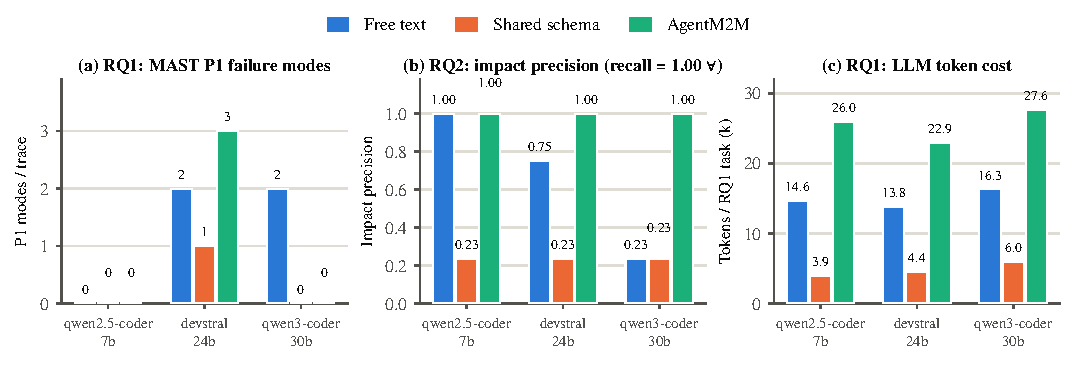
\includegraphics[width=\textwidth]{../evaluation/results/figures/devbench_rq1_rq2_per_model.pdf}
\caption{Per-model breakdown behind Table~\ref{tab:prelim} (RQ1, RQ2;
\code{evaluation/results/csv/devbench\_raw\_metrics\_*.csv} and
\code{devbench\_summary\_*.json}), $n{=}1$ repository (\code{chakin})
$\times$ 3 models. (a) MAST P1 modes per trace: the sign of \tool{}'s
effect flips by model (worse with \code{devstral:24b}, better with
\code{qwen3-coder:30b}, no signal with \code{qwen2.5-coder:7b}).
(b) RQ2 impact precision (recall $=1.00$ for every model/configuration):
\tool{} holds precision $1.00$ for all three models while free text is
non-monotonic in model size. (c) LLM tokens per RQ1 task: \tool{} costs
more than either baseline at this scale.}
\label{fig:prelim}
\end{figure*}

\noindent\textbf{Results.} On \code{chakin}, \emph{no} model/
configuration pair (9 of 9) retained any of the 5 canaries or passed
\code{chakin}'s real acceptance test -- a real, if unencouraging, result at
this scale, not a pipeline defect (a scripted backend that returns
textually correct canary bodies passes 5/5 through the same code path,
confirming the mechanism itself is sound). MAST P1 modes gave a genuinely
mixed, model-dependent signal rather than a clean confirmation or
refutation of Proposition~\ref{prop:struct}: \code{qwen2.5-coder:7b} showed
0 P1 modes for all three configurations (no signal either way);
\code{devstral:24b} showed \emph{more} P1 modes for \tool{} (3) than free
text (2) or shared schema (1) -- the direction Proposition~\ref{prop:struct}
predicts \emph{against}; \code{qwen3-coder:30b} showed \emph{fewer} P1
modes for \tool{} (0) than free text (2), matching shared schema (0) --
the predicted direction. Averaged, \tool{} (1.00) sits between free text
(1.33) and shared schema (0.33): \emph{better than the weakest baseline,
worse than the other, and the ranking flips depending on which single
model is examined} -- an honest summary is that this pilot does not yet
show a consistent P1-reducing effect, in either direction, at $n=1$
repository across 3 models. RQ2 is the one metric where all three models
agree exactly: \tool{}'s $\Obl(\Delta)$ reached recall 1.00 and precision
1.00 on \emph{every one} of the 9 real trials (3 models $\times$ 3 injected
changes), never missing and never over-including -- a structural
consequence of Algorithm 1's stamp check, and the strongest, most
consistent empirical support Proposition~\ref{prop:impact} could plausibly
receive at this scale, precisely because it does not depend on generation
quality. The baselines did not hold as steady: shared-schema's recall 1.00
/ precision $\approx$0.23 (regenerating all 4 real operations) was
identical across all three models, as expected (it makes no LLM calls),
but free-text's precision varied widely and \emph{non-monotonically} with
model size -- 1.00 (\code{qwen2.5-coder:7b}), 0.75 (\code{devstral:24b}),
then 0.23 (\code{qwen3-coder:30b}, essentially indistinguishable from
shared-schema's "list everything" baseline on this run) -- the
\emph{largest} model gave the \emph{least} precise free-text impact
listing of the three, the opposite of what "bigger model, better
free-text reasoning" would predict, on this one repository. RQ3 matched
Proposition-level expectations deterministically and identically for all
three models: the HOT-added Security Reviewer covered all 9 pre-existing
operations (100\% retroactive coverage, 3/3 models) for 7 lines of glue
code, versus an estimated 22 lines the free-text/shared-schema baselines
would need written by hand, once per baseline file, to achieve the same
effect manually -- unsurprising, since retroactive coverage is a structural
property of the match set, not a generation-quality outcome.

\noindent\textbf{Decision rules (fixed before running).} RQ1 is supported only
if the paired 95\% bootstrap interval of the canary-retention difference to the
shared-schema baseline excludes zero and exceeds 10 points, with FM-1.1,
2.2, 2.6 unchanged (negative controls); otherwise it is refuted for this
pilot. At $n=1$ repository this interval is not computable (a paired
bootstrap needs multiple repositories) and canary retention was 0\% for
every configuration and all three models, so RQ1 is reported as
\textbf{inconclusive}, not supported, for this pilot; the negative controls
(FM-1.1, 2.2, 2.6) were unchanged (mostly absent) across configurations for
all three models, consistent with the prediction, but on a null canary
result this is weak evidence, and the P1-mode direction flipped sign
across models (worse for \tool{} with \code{devstral:24b}, better with
\code{qwen3-coder:30b}), so the substantive prediction is neither
confirmed nor cleanly refuted here. Proposition~\ref{prop:impact} gives
recall $1$ only relative to declared footprints; on \code{chakin} every
RQ2 miss category was empty for \tool{} in all three models (precision and
recall both 1.00, 9/9), so there is nothing to attribute to
footprint-versus-annotation cause here -- this is the one part of the
pilot that behaved exactly as predicted, with no exceptions. Threats: as
of this draft, a \textbf{single-repository} result across all three
planned models (10 Python DevBench repositories were planned, then 6 after
observed per-repository latency, currently 1) -- results at this scale
should be read as a pipeline validation with three real data points per
configuration, not a statistically meaningful comparison; a null RQ1
canary result at $n=1$ cannot distinguish "\tool{} has no effect" from
"this pilot is underpowered to detect one"; one baseline set of canaries
and injected changes, authored by us; the MAST annotator is our own
approximation of Cemri et al.'s unreleased tool and, being the same model
being evaluated judging its own transcript, may be miscalibrated for
\tool{}'s non-conversational, per-operation transcript shape relative to
the free-flowing dialogues it was designed to annotate -- two of three
models we tested (\code{qwen2.5-coder:7b}, \code{devstral:24b}) show equal
or \emph{more}, not fewer, P1 modes for \tool{} than free text, matching
our companion SWE-bench-Lite pilot's direction of effect
(\code{evaluation/results/csv/pilot\_table.csv}: 1.40 vs.\ 0.60), while the
third (\code{qwen3-coder:30b}) shows the predicted direction -- this
inconsistency is either a real, model-dependent effect or a sign the
annotator itself needs revisiting for this transcript shape, and at this
sample size we cannot tell which; and, with no human annotator available,
the protocol's 20\% manual re-label and RQ2's manually-labelled impact
sets are replaced by an independent second-model judge (never the model
being judged) and by the declared-footprint oracle above, respectively --
both are disclosed substitutions, not the original protocol.

\subsection{Discussion and limitations}\label{subsec:discussion}

\noindent\textbf{What \tool{} cannot fix.} Modes rooted in a single agent's
reasoning (FM-1.1, 2.2, 2.6) are outside a coordination layer; so is a weak
validator, which Proposition~\ref{prop:error} makes visible rather than
curing. \textbf{Cost of metamodels.} Authoring view metamodels and rules is
the price of the guarantees; its amortization across tasks is an empirical
question (RQ3). \textbf{Expressiveness.} Code is lifted into a coarse
\cls{CodeEdit} view, so Proposition~\ref{prop:impact} is only as fine-grained
as the footprints this view exposes. \textbf{Why not one shared schema?} A shared schema~\cite{zhang2026patchboard}
validates \emph{each} write; \tool{} additionally relates \emph{pairs} of
views, which is what change impact and coverage need
(Propositions~\ref{prop:struct} and~\ref{prop:impact}); the shared-schema
baseline isolates exactly this difference.
\textbf{Relation to LLMs for MDE.} Prior
work uses LLMs \emph{inside} modeling
tasks~\cite{chaaben2023fewshot,chen2023domainmodeling,clariso2023mdpe}; we
invert the direction and use MDE to discipline LLM teams.
\textbf{Sustainability.} Structural rules run without LLM calls and
Proposition~\ref{prop:impact} re-invokes only the bindings in $\Obl(\Delta)$;
on our \code{chakin} pilot (Table~\ref{tab:prelim}), mean tokens per RQ1
task were 14.9k/4.8k/25.5k for free text/shared schema/\tool{}
respectively -- \tool{}'s per-operation \code{@llm} calls cost more tokens
than either baseline at this scale, so its sustainability case rests on
Proposition~\ref{prop:impact}'s change-time savings (RQ2), not on the
initial generation being cheaper; \hyp{we have not yet converted token
counts into an energy estimate.}

\section{Future Plans}\label{sec:future}

To turn this idea into a full paper we will address three research
challenges, in this order, each ending in a falsifiable deliverable. \RC{1}~\emph{Learning the glue:} view metamodels and relation
models are costly to author; we will let an architect agent propose them and
admit a proposal only if it conforms to a meta-metamodel and passes
round-trip checks, mirroring the PIM-to-PSM refinement of
MeTAGeM-Trace~\cite{vara2014metagem}. \RC{2}~\emph{Bidirectionality:}
downstream agents also edit upstream intent (a developer discovers an
infeasible criterion); we will lift hand-offs to bx and characterize
correctness and hippocraticness~\cite{stevens2010qvt} when the backward
direction is stochastic. \RC{3}~\emph{Evidence at scale:} Sec.~\ref{sec:eval}'s
pilot covers 6 of DevBench's 10 Python repositories, one seed, and three
open-weight models; we will extend it to the remaining Python repositories
and to DevBench's Java/C++/JavaScript repositories, add seeds, and
re-implement MetaGPT- and ChatDev-style
teams~\cite{hong2024metagpt,qian2024chatdev} on \tool{} with the same LLMs
and roles, continuing to treat a failure to reduce P1 modes relative to the
shared-schema baseline as refuting our central claim. We will also compare
footprint-bounded against full-context prompting, since
Proposition~\ref{prop:impact} trades context for soundness and the
effect on output quality is unknown. All artifacts will be released.

\section{Data Availability}\label{sec:data}

The MAST mapping with its rationale, the \devteam{} metamodels and rules,
and \hyp{the prototype} are available at \fixme{anonymized link}.

\begin{thebibliography}{99}
\footnotesize

\bibitem{he2025lma}
J.~He, C.~Treude, and D.~Lo, ``LLM-based multi-agent systems for software
engineering: Literature review, vision, and the road ahead,'' \emph{ACM
Trans. Softw. Eng. Methodol.}, vol.~34, no.~5, 2025.

\bibitem{hong2024metagpt}
S.~Hong \emph{et~al.}, ``MetaGPT: Meta programming for a multi-agent
collaborative framework,'' in \emph{Proc. ICLR}, 2024.

\bibitem{qian2024chatdev}
C.~Qian \emph{et~al.}, ``ChatDev: Communicative agents for software
development,'' in \emph{Proc. ACL}, 2024.

\bibitem{tao2024magis}
W.~Tao, Y.~Zhou, Y.~Wang, W.~Zhang, H.~Zhang, and Y.~Cheng, ``MAGIS:
LLM-based multi-agent framework for GitHub issue resolution,'' in
\emph{Proc. NeurIPS}, 2024.

\bibitem{wu2024autogen}
Q.~Wu \emph{et~al.}, ``AutoGen: Enabling next-gen LLM applications via
multi-agent conversation,'' in \emph{Proc. COLM}, 2024.

\bibitem{li2023camel}
G.~Li, H.~A.~A.~K. Hammoud, H.~Itani, D.~Khizbullin, and B.~Ghanem,
``CAMEL: Communicative agents for `mind' exploration of large language model
society,'' in \emph{Proc. NeurIPS}, 2023.

\bibitem{chen2024agentverse}
W.~Chen \emph{et~al.}, ``AgentVerse: Facilitating multi-agent collaboration
and exploring emergent behaviors,'' in \emph{Proc. ICLR}, 2024.

\bibitem{cemri2025mast}
M.~Cemri, M.~Z. Pan, S.~Yang \emph{et~al.}, ``Why do multi-agent LLM systems
fail?'' in \emph{Proc. NeurIPS (Datasets and Benchmarks Track)}, 2025,
arXiv:2503.13657.

\bibitem{mcp2024}
Anthropic, ``Model Context Protocol,'' specification,
\url{https://modelcontextprotocol.io}, 2024.

\bibitem{a2a2025}
Google, ``Agent2Agent (A2A) protocol,'' specification,
\url{https://a2a-protocol.org}, 2025.

\bibitem{zhang2026patchboard}
S.~Zhang, Y.~Shi, J.~Zhang, Y.~Zhao, and L.~Wang, ``PatchBoard:
Schema-grounded state mutation for reliable and auditable LLM multi-agent
collaboration,'' arXiv:2605.29313, 2026.

\bibitem{zhuge2024gptswarm}
M.~Zhuge, W.~Wang, L.~Kirsch, F.~Faccio, D.~Khizbullin, and
J.~Schmidhuber, ``GPTSwarm: Language agents as optimizable graphs,'' in
\emph{Proc. ICML}, 2024.

\bibitem{hu2025adas}
S.~Hu, C.~Lu, and J.~Clune, ``Automated design of agentic systems,'' in
\emph{Proc. ICLR}, 2025.

\bibitem{zhang2025aflow}
J.~Zhang \emph{et~al.}, ``AFlow: Automating agentic workflow generation,''
in \emph{Proc. ICLR}, 2025.

\bibitem{klare2021vitruvius}
H.~Klare, M.~E. Kramer, M.~Langhammer, D.~Werle, E.~Burger, and
R.~Reussner, ``Enabling consistency in view-based system development---The
Vitruvius approach,'' \emph{J. Syst. Softw.}, vol.~171, p.~110815, 2021.

\bibitem{bruneliere2019views}
H.~Bruneliere, E.~Burger, J.~Cabot, and M.~Wimmer, ``A feature-based survey
of model view approaches,'' \emph{Softw. Syst. Model.}, vol.~18, no.~3,
pp.~1931--1952, 2019.

\bibitem{czarnecki2009bx}
K.~Czarnecki, J.~N. Foster, Z.~Hu, R.~L{\"a}mmel, A.~Sch{\"u}rr, and
J.~F. Terwilliger, ``Bidirectional transformations: A cross-discipline
perspective,'' in \emph{Proc. ICMT}, LNCS 5563, 2009, pp.~260--283.

\bibitem{stevens2010qvt}
P.~Stevens, ``Bidirectional model transformations in QVT: Semantic issues
and open questions,'' \emph{Softw. Syst. Model.}, vol.~9, no.~1, pp.~7--20,
2010.

\bibitem{stevens2020networks}
P.~Stevens, ``Maintaining consistency in networks of models: Bidirectional
transformations in the large,'' \emph{Softw. Syst. Model.}, vol.~19, no.~1,
pp.~39--65, 2020.

\bibitem{klare2023termination}
H.~Klare and J.~Gleitze, ``Termination and expressiveness of execution
strategies for networks of bidirectional model transformations,''
\emph{Formal Asp. Comput.}, vol.~35, no.~3, pp.~15:1--15:35, 2023.

\bibitem{blair2009runtime}
G.~Blair, N.~Bencomo, and R.~B. France, ``Models@run.time,''
\emph{Computer}, vol.~42, no.~10, pp.~22--27, 2009.

\bibitem{tisi2009hot}
M.~Tisi, F.~Jouault, P.~Fraternali, S.~Ceri, and J.~B{\'e}zivin, ``On the
use of higher-order model transformations,'' in \emph{Proc. ECMDA-FA}, LNCS
5562, 2009, pp.~18--33.

\bibitem{jouault2008atl}
F.~Jouault, F.~Allilaire, J.~B{\'e}zivin, and I.~Kurtev, ``ATL: A model
transformation tool,'' \emph{Sci. Comput. Program.}, vol.~72, no.~1--2,
pp.~31--39, 2008.

\bibitem{jouault2005traceability}
F.~Jouault, ``Loosely coupled traceability for ATL,'' in \emph{Proc. ECMDA
Workshop on Traceability}, 2005.

\bibitem{vara2014metagem}
J.~M. Vara, V.~A. Bollati, {\'A}.~Jim{\'e}nez, and E.~Marcos, ``Dealing with
traceability in the MDD of model transformations,'' \emph{IEEE Trans. Softw.
Eng.}, vol.~40, no.~6, pp.~555--583, 2014.

\bibitem{chaaben2023fewshot}
M.~Ben~Chaaben, L.~Burgue{\~n}o, and H.~Sahraoui, ``Towards using few-shot
prompt learning for automating model completion,'' in \emph{Proc.
ICSE-NIER}, 2023, pp.~7--12.

\bibitem{chen2023domainmodeling}
K.~Chen, Y.~Yang, B.~Chen, J.~A. Hern{\'a}ndez~L{\'o}pez, G.~Mussbacher,
and D.~Varr{\'o}, ``Automated domain modeling with large language models: A
comparative study,'' in \emph{Proc. MODELS}, 2023, pp.~162--172.

\bibitem{clariso2023mdpe}
R.~Claris{\'o} and J.~Cabot, ``Model-driven prompt engineering,'' in
\emph{Proc. MODELS}, 2023.

\bibitem{li2024devbench}
B.~Li, W.~Wu, Z.~Tang, L.~Shi, J.~Yang, J.~Li, S.~Yao, C.~Qian, B.~Hui,
Q.~Zhang, Z.~Yu, H.~Du, P.~Yang, D.~Lin, C.~Peng, and K.~Chen, ``DevBench:
A comprehensive benchmark for software development,'' arXiv:2403.08604,
2024.

\bibitem{hui2024qwen25coder}
B.~Hui \emph{et~al.}, ``Qwen2.5-Coder technical report,'' arXiv:2409.12186,
2024.

\bibitem{mistral2025devstral}
Mistral AI and All Hands AI, ``Devstral: Fine-tuning language models for
coding agent applications,'' arXiv:2509.25193, 2025.

\bibitem{qwen2025qwen3}
A.~Yang \emph{et~al.}, ``Qwen3 technical report,'' arXiv:2505.09388, 2025.

\end{thebibliography}

\end{document}